\renewcommand{\appendixname}{APPENDIX}
\appendix
%%% Правка оформления ссылок на приложения:
%http://tex.stackexchange.com/questions/56839/chaptername-is-used-even-for-appendix-chapters-in-toc
%http://tex.stackexchange.com/questions/59349/table-of-contents-with-chapter-and-appendix
%% требует двойной компиляции
%\addtocontents{toc}{\def\protect\cftchappresnum{\appendixname{} }%
%\setlength{\cftchapnumwidth}{\widthof{\cftchapfont\appendixname\cftchapaftersnum}}%
%}
%% Оформление заголовков приложений ближе к ГОСТ:
\sectionformat{\chapter}[display]{% Параметры заголовков разделов в тексте
    label=\appendixname\ \thechapter,% (ГОСТ Р 2.105, 4.3.6)
    labelsep=20pt,
}
%\renewcommand\thechapter{\Asbuk{chapter}} % Чтобы приложения русскими буквами нумеровались

\chapter{Appendix} \label{AppendixA}

%Для крупных листингов есть два способа. Первый красивый, но в нём могут быть проблемы с поддержкой кириллицы (у вас может встречаться в комментариях и
%печатаемых сообщениях), он представлен на листинге~\ref{list:hwbeauty}.
%%\renewcommand\FBbskip{-20pt} % если хотим притянуть что-то к плавающему окружению из floatrow
%\begin{ListingEnv}[H]% буква H означает Here, ставим здесь,
%    % элементы, которые нежелательно разрывать обычно не ставят
%    % посреди страницы: вместо H используется t (top, сверху страницы),
%    % или b (bottom) или p (page, на отдельной странице)
%%    \captionsetup{format=tablenocaption}% должен стоять до самого caption
%%    \thisfloatsetup{\capposition=top}%
%    \caption{Программа “Hello, world” на \protect\cpp}
%    % далее метка для ссылки:
%    \label{list:hwbeauty}
%    % окружение учитывает пробелы и табляции и приеняет их в сответсвии с настройкми
%    \begin{lstlisting}[language={[ISO]C++}]
%	#include <iostream>
%	using namespace std;
%
%	int main() //кириллица в комментариях при xelatex и lualatex имеет проблемы с пробелами
%	{
%		cout << "Hello, world" << endl; //latin letters in commentaries
%		system("pause");
%		return 0;
%	}
%    \end{lstlisting}
%\end{ListingEnv}%
%Второй не такой красивый, но без ограничений (см.~листинг~\ref{list:hwplain}).
%\begin{ListingEnv}[H]
%    \begin{Verb}
%        
%        #include <iostream>
%        using namespace std;
%        
%        int main() //кириллица в комментариях
%        {
%            cout << "Привет, мир" << endl;
%        }
%    \end{Verb}
%    \caption{Программа “Hello, world” без подсветки}
%    \label{list:hwplain}
%\end{ListingEnv}
%
%Можно использовать первый для вставки небольших фрагментов
%внутри текста, а второй для вставки полного
%кода в приложении, если таковое имеется.
%
%Если нужно вставить совсем короткий пример кода (одна или две строки), то выделение  линейками и нумерация может смотреться чересчур громоздко. В таких случаях можно использовать окружения \texttt{lstlisting} или \texttt{Verb} без \texttt{ListingEnv}. Приведём такой пример с указанием языка программирования, отличного от заданного по умолчанию:
%\begin{lstlisting}[language=Haskell]
%fibs = 0 : 1 : zipWith (+) fibs (tail fibs)
%\end{lstlisting}
%Такое решение~--- со вставкой нумерованных листингов покрупнее
%и вставок без выделения для маленьких фрагментов~--- выбрано,
%например, в книге Эндрю Таненбаума и Тодда Остина по архитектуре
%%компьютера~\autocite{TanAus2013} (см.~рис.~\ref{fig:tan-aus}).
%
%Наконец, для оформления идентификаторов внутри строк
%(функция \lstinline{main} и тому подобное) используется
%\texttt{lstinline} или, самое простое, моноширинный текст
%(\texttt{\textbackslash texttt}).
%
%
%Пример~\ref{list:internal3}, иллюстрирующий подключение переопределённого языка. Может быть полезным, если подсветка кода работает криво. Без дополнительного окружения, с подписью и ссылкой, реализованной встроенным средством.
%\begin{lstlisting}[language={Renhanced},caption={Пример листинга c подписью собственными средствами},label={list:internal3}]
%## Caching the Inverse of a Matrix
%
%## Matrix inversion is usually a costly computation and there may be some
%## benefit to caching the inverse of a matrix rather than compute it repeatedly
%## This is a pair of functions that cache the inverse of a matrix.
%
%## makeCacheMatrix creates a special "matrix" object that can cache its inverse
%
%makeCacheMatrix <- function(x = matrix()) {#кириллица в комментариях при xelatex b lualatex имеет проблемы с пробелами
%    i <- NULL
%    set <- function(y) {
%        x <<- y
%        i <<- NULL
%    }
%    get <- function() x
%    setSolved <- function(solve) i <<- solve
%    getSolved <- function() i
%    list(set = set, get = get,
%    setSolved = setSolved,
%    getSolved = getSolved)
%    
%}
%
%
%## cacheSolve computes the inverse of the special "matrix" returned by
%## makeCacheMatrix above. If the inverse has already been calculated (and the
%## matrix has not changed), then the cachesolve should retrieve the inverse from
%## the cache.
%
%cacheSolve <- function(x, ...) {
%    ## Return a matrix that is the inverse of 'x'
%    i <- x$getSolved()
%    if(!is.null(i)) {
%        message("getting cached data")
%        return(i)
%    }
%    data <- x$get()
%    i <- solve(data, ...)
%    x$setSolved(i)
%    i  
%}
%\end{lstlisting}
%
%Листинг~\ref{list:external1} подгружается из внешнего файла. Приходится загружать без окружения дополнительного. Иначе по страницам не переносится.
%    \lstinputlisting[lastline=78,language={R},caption={Листинг из внешнего файла},label={list:external1}]{./listings/run_analysis.R}
%
%
%
%
%
%
%\chapter{Очень длинное название второго приложения, в котором продемонстрирована работа с длинными таблицами} \label{AppendixB}
%
% \section{Подраздел приложения}\label{AppendixB1}
%Вот размещается длинная таблица:
%\fontsize{10pt}{10pt}\selectfont
%\begin{longtable}[c]{|l|c|l|l|}
%% \caption{Описание входных файлов модели}\label{Namelists} 
%%\\ 
% \hline
% %\multicolumn{4}{|c|}{\textbf{Файл puma\_namelist}}        \\ \hline
% Параметр & Умолч. & Тип & Описание               \\ \hline
%                                              \endfirsthead   \hline
% \multicolumn{4}{|c|}{\small\slshape (продолжение)}        \\ \hline
% Параметр & Умолч. & Тип & Описание               \\ \hline
%                                              \endhead        \hline
% \multicolumn{4}{|r|}{\small\slshape продолжение следует}  \\ \hline
%                                              \endfoot        \hline
%                                              \endlastfoot
% \multicolumn{4}{|l|}{\&INP}        \\ \hline 
% kick & 1 & int & 0: инициализация без шума ($p_s = const$) \\
%      &   &     & 1: генерация белого шума                  \\
%      &   &     & 2: генерация белого шума симметрично относительно \\
%  & & & экватора    \\
% mars & 0 & int & 1: инициализация модели для планеты Марс     \\
% kick & 1 & int & 0: инициализация без шума ($p_s = const$) \\
%      &   &     & 1: генерация белого шума                  \\
%      &   &     & 2: генерация белого шума симметрично относительно \\
%  & & & экватора    \\
% mars & 0 & int & 1: инициализация модели для планеты Марс     \\
%kick & 1 & int & 0: инициализация без шума ($p_s = const$) \\
%      &   &     & 1: генерация белого шума                  \\
%      &   &     & 2: генерация белого шума симметрично относительно \\
%  & & & экватора    \\
% mars & 0 & int & 1: инициализация модели для планеты Марс     \\
%kick & 1 & int & 0: инициализация без шума ($p_s = const$) \\
%      &   &     & 1: генерация белого шума                  \\
%      &   &     & 2: генерация белого шума симметрично относительно \\
%  & & & экватора    \\
% mars & 0 & int & 1: инициализация модели для планеты Марс     \\
%kick & 1 & int & 0: инициализация без шума ($p_s = const$) \\
%      &   &     & 1: генерация белого шума                  \\
%      &   &     & 2: генерация белого шума симметрично относительно \\
%  & & & экватора    \\
% mars & 0 & int & 1: инициализация модели для планеты Марс     \\
%kick & 1 & int & 0: инициализация без шума ($p_s = const$) \\
%      &   &     & 1: генерация белого шума                  \\
%      &   &     & 2: генерация белого шума симметрично относительно \\
%  & & & экватора    \\
% mars & 0 & int & 1: инициализация модели для планеты Марс     \\
%kick & 1 & int & 0: инициализация без шума ($p_s = const$) \\
%      &   &     & 1: генерация белого шума                  \\
%      &   &     & 2: генерация белого шума симметрично относительно \\
%  & & & экватора    \\
% mars & 0 & int & 1: инициализация модели для планеты Марс     \\
%kick & 1 & int & 0: инициализация без шума ($p_s = const$) \\
%      &   &     & 1: генерация белого шума                  \\
%      &   &     & 2: генерация белого шума симметрично относительно \\
%  & & & экватора    \\
% mars & 0 & int & 1: инициализация модели для планеты Марс     \\
%kick & 1 & int & 0: инициализация без шума ($p_s = const$) \\
%      &   &     & 1: генерация белого шума                  \\
%      &   &     & 2: генерация белого шума симметрично относительно \\
%  & & & экватора    \\
% mars & 0 & int & 1: инициализация модели для планеты Марс     \\
%kick & 1 & int & 0: инициализация без шума ($p_s = const$) \\
%      &   &     & 1: генерация белого шума                  \\
%      &   &     & 2: генерация белого шума симметрично относительно \\
%  & & & экватора    \\
% mars & 0 & int & 1: инициализация модели для планеты Марс     \\
%kick & 1 & int & 0: инициализация без шума ($p_s = const$) \\
%      &   &     & 1: генерация белого шума                  \\
%      &   &     & 2: генерация белого шума симметрично относительно \\
%  & & & экватора    \\
% mars & 0 & int & 1: инициализация модели для планеты Марс     \\
%kick & 1 & int & 0: инициализация без шума ($p_s = const$) \\
%      &   &     & 1: генерация белого шума                  \\
%      &   &     & 2: генерация белого шума симметрично относительно \\
%  & & & экватора    \\
% mars & 0 & int & 1: инициализация модели для планеты Марс     \\
%kick & 1 & int & 0: инициализация без шума ($p_s = const$) \\
%      &   &     & 1: генерация белого шума                  \\
%      &   &     & 2: генерация белого шума симметрично относительно \\
%  & & & экватора    \\
% mars & 0 & int & 1: инициализация модели для планеты Марс     \\
%kick & 1 & int & 0: инициализация без шума ($p_s = const$) \\
%      &   &     & 1: генерация белого шума                  \\
%      &   &     & 2: генерация белого шума симметрично относительно \\
%  & & & экватора    \\
% mars & 0 & int & 1: инициализация модели для планеты Марс     \\
%kick & 1 & int & 0: инициализация без шума ($p_s = const$) \\
%      &   &     & 1: генерация белого шума                  \\
%      &   &     & 2: генерация белого шума симметрично относительно \\
%  & & & экватора    \\
% mars & 0 & int & 1: инициализация модели для планеты Марс     \\
% \hline
%  %& & & $\:$ \\ 
% \multicolumn{4}{|l|}{\&SURFPAR}        \\ \hline
%kick & 1 & int & 0: инициализация без шума ($p_s = const$) \\
%      &   &     & 1: генерация белого шума                  \\
%      &   &     & 2: генерация белого шума симметрично относительно \\
%  & & & экватора    \\
% mars & 0 & int & 1: инициализация модели для планеты Марс     \\
%kick & 1 & int & 0: инициализация без шума ($p_s = const$) \\
%      &   &     & 1: генерация белого шума                  \\
%      &   &     & 2: генерация белого шума симметрично относительно \\
%  & & & экватора    \\
% mars & 0 & int & 1: инициализация модели для планеты Марс     \\
%kick & 1 & int & 0: инициализация без шума ($p_s = const$) \\
%      &   &     & 1: генерация белого шума                  \\
%      &   &     & 2: генерация белого шума симметрично относительно \\
%  & & & экватора    \\
% mars & 0 & int & 1: инициализация модели для планеты Марс     \\
%kick & 1 & int & 0: инициализация без шума ($p_s = const$) \\
%      &   &     & 1: генерация белого шума                  \\
%      &   &     & 2: генерация белого шума симметрично относительно \\
%  & & & экватора    \\
% mars & 0 & int & 1: инициализация модели для планеты Марс     \\
%kick & 1 & int & 0: инициализация без шума ($p_s = const$) \\
%      &   &     & 1: генерация белого шума                  \\
%      &   &     & 2: генерация белого шума симметрично относительно \\
%  & & & экватора    \\
% mars & 0 & int & 1: инициализация модели для планеты Марс     \\
%kick & 1 & int & 0: инициализация без шума ($p_s = const$) \\
%      &   &     & 1: генерация белого шума                  \\
%      &   &     & 2: генерация белого шума симметрично относительно \\
%  & & & экватора    \\
% mars & 0 & int & 1: инициализация модели для планеты Марс     \\
%kick & 1 & int & 0: инициализация без шума ($p_s = const$) \\
%      &   &     & 1: генерация белого шума                  \\
%      &   &     & 2: генерация белого шума симметрично относительно \\
%  & & & экватора    \\
% mars & 0 & int & 1: инициализация модели для планеты Марс     \\
%kick & 1 & int & 0: инициализация без шума ($p_s = const$) \\
%      &   &     & 1: генерация белого шума                  \\
%      &   &     & 2: генерация белого шума симметрично относительно \\
%  & & & экватора    \\
% mars & 0 & int & 1: инициализация модели для планеты Марс     \\
%kick & 1 & int & 0: инициализация без шума ($p_s = const$) \\
%      &   &     & 1: генерация белого шума                  \\
%      &   &     & 2: генерация белого шума симметрично относительно \\
%  & & & экватора    \\
% mars & 0 & int & 1: инициализация модели для планеты Марс     \\ 
% \hline 
%\end{longtable}
%
%\normalsize% возвращаем шрифт к нормальному
%\section{Ещё один подраздел приложения} \label{AppendixB2}
%
%Нужно больше подразделов приложения!
%
%Пример длинной таблицы с записью продолжения по ГОСТ 2.105
%
%    \centering
%	\small
%    \begin{longtable}[c]{|l|c|l|l|}
%	\caption{Наименование таблицы средней длины}%
%    \label{tbl:test5}% label всегда желательно идти после caption
%    \\ 
%    \hline
%     %\multicolumn{4}{|c|}{\textbf{Файл puma\_namelist}}        \\ \hline
%     Параметр & Умолч. & Тип & Описание               \\ \hline
%                                                  \endfirsthead
%%     \multicolumn{4}{|c|}{\small\slshape (продолжение)}        \\ \hline
% \captionsetup{format=tablenocaption,labelformat=continued}% должен стоять до самого caption
% \caption[]{} \\
%    \hline
%     Параметр & Умолч. & Тип & Описание               \\ \hline
%                                                  \endhead        \hline
%%     \multicolumn{4}{|r|}{\small\slshape продолжение следует}  \\
%%\hline
%                                                  \endfoot        \hline
%                                                  \endlastfoot
%     \multicolumn{4}{|l|}{\&INP}        \\ \hline 
%     kick & 1 & int & 0: инициализация без шума ($p_s = const$) \\
%          &   &     & 1: генерация белого шума                  \\
%          &   &     & 2: генерация белого шума симметрично относительно \\
%      & & & экватора    \\
%     mars & 0 & int & 1: инициализация модели для планеты Марс     \\
%     kick & 1 & int & 0: инициализация без шума ($p_s = const$) \\
%          &   &     & 1: генерация белого шума                  \\
%          &   &     & 2: генерация белого шума симметрично относительно \\
%      & & & экватора    \\
%     mars & 0 & int & 1: инициализация модели для планеты Марс     \\
%    kick & 1 & int & 0: инициализация без шума ($p_s = const$) \\
%          &   &     & 1: генерация белого шума                  \\
%          &   &     & 2: генерация белого шума симметрично относительно \\
%      & & & экватора    \\
%     mars & 0 & int & 1: инициализация модели для планеты Марс     \\
%    kick & 1 & int & 0: инициализация без шума ($p_s = const$) \\
%          &   &     & 1: генерация белого шума                  \\
%          &   &     & 2: генерация белого шума симметрично относительно \\
%      & & & экватора    \\
%     mars & 0 & int & 1: инициализация модели для планеты Марс     \\
%    kick & 1 & int & 0: инициализация без шума ($p_s = const$) \\
%          &   &     & 1: генерация белого шума                  \\
%          &   &     & 2: генерация белого шума симметрично относительно \\
%      & & & экватора    \\
%     mars & 0 & int & 1: инициализация модели для планеты Марс     \\
%    kick & 1 & int & 0: инициализация без шума ($p_s = const$) \\
%          &   &     & 1: генерация белого шума                  \\
%          &   &     & 2: генерация белого шума симметрично относительно \\
%      & & & экватора    \\
%     mars & 0 & int & 1: инициализация модели для планеты Марс     \\
%    kick & 1 & int & 0: инициализация без шума ($p_s = const$) \\
%          &   &     & 1: генерация белого шума                  \\
%          &   &     & 2: генерация белого шума симметрично относительно \\
%      & & & экватора    \\
%     mars & 0 & int & 1: инициализация модели для планеты Марс     \\
%    kick & 1 & int & 0: инициализация без шума ($p_s = const$) \\
%          &   &     & 1: генерация белого шума                  \\
%          &   &     & 2: генерация белого шума симметрично относительно \\
%      & & & экватора    \\
%     mars & 0 & int & 1: инициализация модели для планеты Марс     \\
%    kick & 1 & int & 0: инициализация без шума ($p_s = const$) \\
%          &   &     & 1: генерация белого шума                  \\
%          &   &     & 2: генерация белого шума симметрично относительно \\
%      & & & экватора    \\
%     mars & 0 & int & 1: инициализация модели для планеты Марс     \\
%    kick & 1 & int & 0: инициализация без шума ($p_s = const$) \\
%          &   &     & 1: генерация белого шума                  \\
%          &   &     & 2: генерация белого шума симметрично относительно \\
%      & & & экватора    \\
%     mars & 0 & int & 1: инициализация модели для планеты Марс     \\
%    kick & 1 & int & 0: инициализация без шума ($p_s = const$) \\
%          &   &     & 1: генерация белого шума                  \\
%          &   &     & 2: генерация белого шума симметрично относительно \\
%      & & & экватора    \\
%     mars & 0 & int & 1: инициализация модели для планеты Марс     \\
%    kick & 1 & int & 0: инициализация без шума ($p_s = const$) \\
%          &   &     & 1: генерация белого шума                  \\
%          &   &     & 2: генерация белого шума симметрично относительно \\
%      & & & экватора    \\
%     mars & 0 & int & 1: инициализация модели для планеты Марс     \\
%    kick & 1 & int & 0: инициализация без шума ($p_s = const$) \\
%          &   &     & 1: генерация белого шума                  \\
%          &   &     & 2: генерация белого шума симметрично относительно \\
%      & & & экватора    \\
%     mars & 0 & int & 1: инициализация модели для планеты Марс     \\
%    kick & 1 & int & 0: инициализация без шума ($p_s = const$) \\
%          &   &     & 1: генерация белого шума                  \\
%          &   &     & 2: генерация белого шума симметрично относительно \\
%      & & & экватора    \\
%     mars & 0 & int & 1: инициализация модели для планеты Марс     \\
%    kick & 1 & int & 0: инициализация без шума ($p_s = const$) \\
%          &   &     & 1: генерация белого шума                  \\
%          &   &     & 2: генерация белого шума симметрично относительно \\
%      & & & экватора    \\
%     mars & 0 & int & 1: инициализация модели для планеты Марс     \\
%     \hline
%      %& & & $\:$ \\ 
%     \multicolumn{4}{|l|}{\&SURFPAR}        \\ \hline
%    kick & 1 & int & 0: инициализация без шума ($p_s = const$) \\
%          &   &     & 1: генерация белого шума                  \\
%          &   &     & 2: генерация белого шума симметрично относительно \\
%      & & & экватора    \\
%     mars & 0 & int & 1: инициализация модели для планеты Марс     \\
%    kick & 1 & int & 0: инициализация без шума ($p_s = const$) \\
%          &   &     & 1: генерация белого шума                  \\
%          &   &     & 2: генерация белого шума симметрично относительно \\
%      & & & экватора    \\
%     mars & 0 & int & 1: инициализация модели для планеты Марс     \\
%    kick & 1 & int & 0: инициализация без шума ($p_s = const$) \\
%          &   &     & 1: генерация белого шума                  \\
%          &   &     & 2: генерация белого шума симметрично относительно \\
%      & & & экватора    \\
%     mars & 0 & int & 1: инициализация модели для планеты Марс     \\
%    kick & 1 & int & 0: инициализация без шума ($p_s = const$) \\
%          &   &     & 1: генерация белого шума                  \\
%          &   &     & 2: генерация белого шума симметрично относительно \\
%      & & & экватора    \\
%     mars & 0 & int & 1: инициализация модели для планеты Марс     \\
%    kick & 1 & int & 0: инициализация без шума ($p_s = const$) \\
%          &   &     & 1: генерация белого шума                  \\
%          &   &     & 2: генерация белого шума симметрично относительно \\
%      & & & экватора    \\
%     mars & 0 & int & 1: инициализация модели для планеты Марс     \\
%    kick & 1 & int & 0: инициализация без шума ($p_s = const$) \\
%          &   &     & 1: генерация белого шума                  \\
%          &   &     & 2: генерация белого шума симметрично относительно \\
%      & & & экватора    \\
%     mars & 0 & int & 1: инициализация модели для планеты Марс     \\
%    kick & 1 & int & 0: инициализация без шума ($p_s = const$) \\
%          &   &     & 1: генерация белого шума                  \\
%          &   &     & 2: генерация белого шума симметрично относительно \\
%      & & & экватора    \\
%     mars & 0 & int & 1: инициализация модели для планеты Марс     \\
%    kick & 1 & int & 0: инициализация без шума ($p_s = const$) \\
%          &   &     & 1: генерация белого шума                  \\
%          &   &     & 2: генерация белого шума симметрично относительно \\
%      & & & экватора    \\
%     mars & 0 & int & 1: инициализация модели для планеты Марс     \\
%    kick & 1 & int & 0: инициализация без шума ($p_s = const$) \\
%          &   &     & 1: генерация белого шума                  \\
%          &   &     & 2: генерация белого шума симметрично относительно \\
%      & & & экватора    \\
%     mars & 0 & int & 1: инициализация модели для планеты Марс     \\ 
%     \hline 
%    \end{longtable}
%\normalsize% возвращаем шрифт к нормальному
%\section{Очередной подраздел приложения} \label{AppendixB3}
%
%Нужно больше подразделов приложения!
%
%\section{И ещё один подраздел приложения} \label{AppendixB4}
%
%Нужно больше подразделов приложения!
%

\begin{figure}[ht] 
	\center
	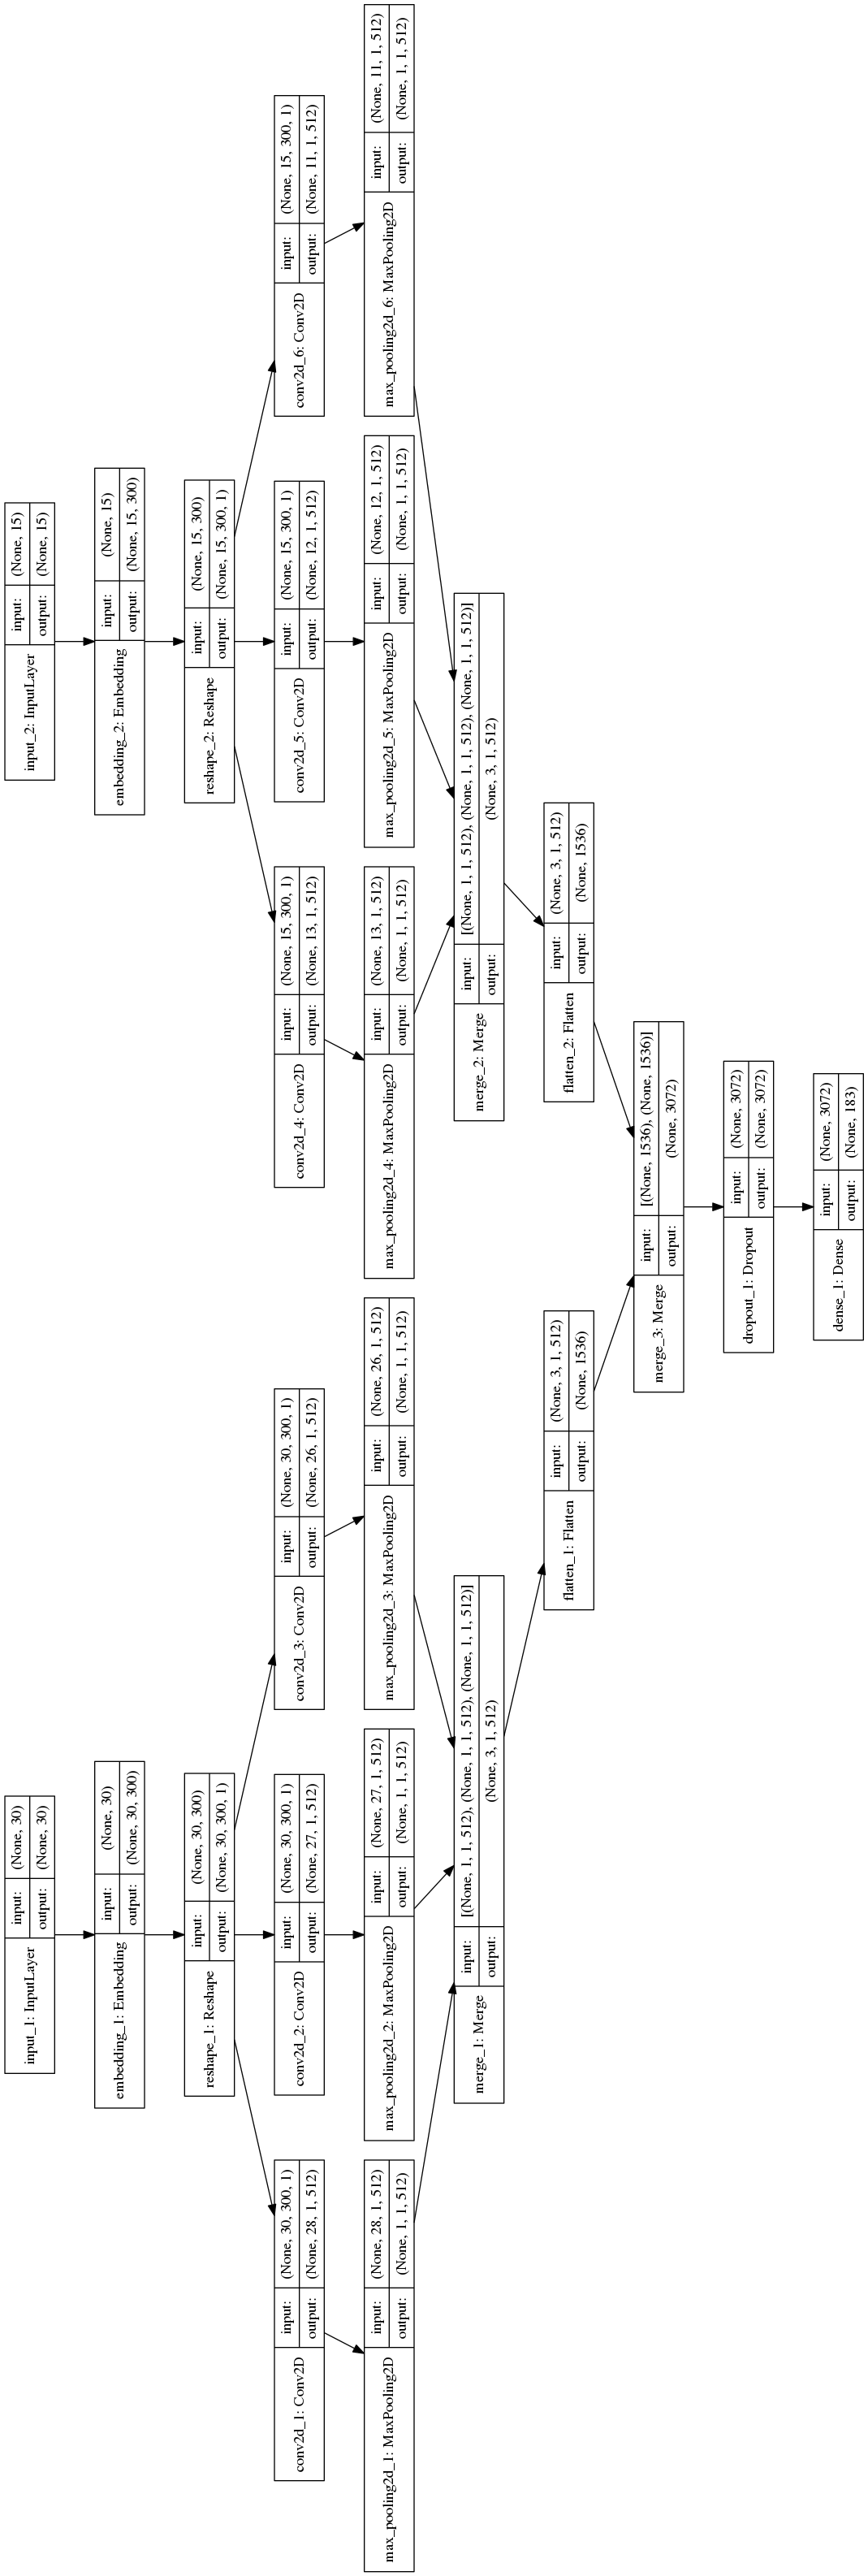
\includegraphics [scale=0.2] {part4/cnn_architecture.png}
	\label{img:cnn_architecture}  
	\caption{Architectures of CNN model} 
\end{figure}



\begin{longtable}[c]{|l|c|c|l|l|}
	\caption[Classification report]{Classification report}
	\label{tab:amortecimentos}\\
	\hline  category & precision & recall &  f1-score & support\\ \hline
	\endhead
	\hline
	\endlastfoot
	
	1        & 0         & 0      & 0        & 7       \\
	3        & 0         & 0      & 0        & 4       \\
	4        & 0         & 0      & 0        & 2       \\
	5        & 0         & 0      & 0        & 1       \\
	6        & 0         & 0      & 0        & 6       \\
	7        & 0         & 0      & 0        & 1       \\
	8        & 0         & 0      & 0        & 2       \\
	9        & 0         & 0      & 0        & 2       \\
	11       & 0.78      & 0.58   & 0.66     & 623     \\
	12       & 0.63      & 0.42   & 0.5      & 281     \\
	14       & 0.93      & 0.99   & 0.96     & 8070    \\
	15       & 0.82      & 0.68   & 0.74     & 362     \\
	16       & 0.93      & 0.95   & 0.94     & 1656    \\
	17       & 0.81      & 0.88   & 0.84     & 550     \\
	18       & 0.73      & 0.73   & 0.73     & 314     \\
	19       & 0.82      & 0.9    & 0.86     & 263     \\
	20       & 0.82      & 0.91   & 0.86     & 1151    \\
	21       & 0.91      & 0.41   & 0.56     & 76      \\
	22       & 0.82      & 0.85   & 0.83     & 830     \\
	23       & 0.44      & 0.56   & 0.49     & 482     \\
	24       & 0         & 0      & 0        & 4       \\
	25       & 0.75      & 0.9    & 0.82     & 1910    \\
	26       & 0.76      & 0.84   & 0.8      & 310     \\
	27       & 0         & 0      & 0        & 5       \\
	29       & 0.97      & 0.99   & 0.98     & 12346   \\
	30       & 0.86      & 0.61   & 0.72     & 270     \\
	31       & 0.85      & 0.52   & 0.64     & 224     \\
	33       & 0.9       & 0.95   & 0.92     & 434     \\
	34       & 0.5       & 0.04   & 0.07     & 26      \\
	35       & 0.09      & 0.04   & 0.06     & 24      \\
	36       & 0.16      & 0.15   & 0.16     & 67      \\
	37       & 0.89      & 0.66   & 0.76     & 197     \\
	38       & 0.68      & 0.21   & 0.33     & 183     \\
	40       & 0.81      & 0.68   & 0.74     & 678     \\
	42       & 0.89      & 0.9    & 0.89     & 1298    \\
	43       & 0.71      & 0.81   & 0.76     & 782     \\
	44       & 0.84      & 0.95   & 0.89     & 1184    \\
	45       & 1         & 0.03   & 0.06     & 30      \\
	46       & 0.58      & 0.31   & 0.41     & 181     \\
	47       & 0         & 0      & 0        & 1       \\
	51       & 0.72      & 0.85   & 0.78     & 591     \\
	53       & 0.59      & 0.72   & 0.65     & 793     \\
	55       & 0.84      & 0.95   & 0.89     & 2471    \\
	56       & 0.63      & 0.59   & 0.61     & 537     \\
	57       & 0.86      & 0.72   & 0.79     & 163     \\
	59       & 0         & 0      & 0        & 2       \\
	60       & 0.67      & 0.59   & 0.63     & 231     \\
	61       & 0.7       & 0.5    & 0.58     & 113     \\
	62       & 0.63      & 0.58   & 0.6      & 67      \\
	64       & 1         & 0.79   & 0.88     & 14      \\
	65       & 0.76      & 0.44   & 0.55     & 117     \\
	66       & 1         & 0.21   & 0.35     & 28      \\
	67       & 0.52      & 0.37   & 0.43     & 122     \\
	70       & 0         & 0      & 0        & 4       \\
	71       & 0         & 0      & 0        & 22      \\
	72       & 0.75      & 0.19   & 0.31     & 31      \\
	73       & 0         & 0      & 0        & 1       \\
	74       & 0.59      & 0.73   & 0.65     & 146     \\
	75       & 0         & 0      & 0        & 3       \\
	76       & 0         & 0      & 0        & 18      \\
	78       & 0.57      & 0.75   & 0.65     & 83      \\
	79       & 0.38      & 0.4    & 0.39     & 92      \\
	80       & 0.2       & 0.1    & 0.13     & 21      \\
	81       & 0         & 0      & 0        & 6       \\
	82       & 0.22      & 0.64   & 0.32     & 85      \\
	83       & 0.49      & 0.53   & 0.51     & 78      \\
	84       & 0.24      & 0.25   & 0.24     & 16      \\
	85       & 0.68      & 0.61   & 0.64     & 87      \\
	86       & 0.57      & 0.53   & 0.55     & 32      \\
	87       & 0.2       & 0.14   & 0.17     & 7       \\
	88       & 0         & 0      & 0        & 1       \\
	89       & 0.75      & 0.33   & 0.46     & 27      \\
	90       & 0.53      & 0.47   & 0.5      & 49      \\
	91       & 0.63      & 0.39   & 0.48     & 83      \\
	92       & 0.58      & 0.28   & 0.38     & 25      \\
	93       & 0.42      & 0.29   & 0.34     & 52      \\
	94       & 0         & 0      & 0        & 12      \\
	95       & 0.5       & 0.18   & 0.27     & 11      \\
	96       & 0.65      & 0.48   & 0.55     & 23      \\
	97       & 0         & 0      & 0        & 4       \\
	98       & 0.2       & 0.12   & 0.15     & 17      \\
	99       & 0         & 0      & 0        & 5       \\
	100      & 0.43      & 0.11   & 0.18     & 107     \\
	101      & 0.36      & 0.21   & 0.27     & 47      \\
	102      & 0.22      & 0.11   & 0.15     & 18      \\
	103      & 0         & 0      & 0        & 7       \\
	104      & 0.56      & 0.6    & 0.58     & 47      \\
	105      & 0.46      & 0.6    & 0.52     & 10      \\
	106      & 0         & 0      & 0        & 3       \\
	107      & 0.8       & 0.6    & 0.69     & 68      \\
	108      & 0.71      & 0.14   & 0.23     & 37      \\
	109      & 0.09      & 0.04   & 0.06     & 73      \\
	110      & 0         & 0      & 0        & 1       \\
	111      & 0.79      & 0.75   & 0.77     & 88      \\
	112      & 0.68      & 0.38   & 0.49     & 50      \\
	113      & 0.76      & 0.61   & 0.68     & 83      \\
	114      & 0.78      & 0.64   & 0.7      & 11      \\
	115      & 0.39      & 0.64   & 0.49     & 194     \\
	116      & 0.58      & 0.52   & 0.55     & 87      \\
	117      & 0.41      & 0.33   & 0.37     & 21      \\
	118      & 0.81      & 0.73   & 0.77     & 237     \\
	119      & 0.63      & 0.63   & 0.63     & 70      \\
	120      & 0.67      & 0.56   & 0.61     & 18      \\
	121      & 0         & 0      & 0        & 4       \\
	122      & 0.6       & 0.54   & 0.57     & 28      \\
	123      & 0.55      & 0.89   & 0.68     & 63      \\
	124      & 0.74      & 0.84   & 0.78     & 87      \\
	125      & 0.65      & 0.57   & 0.61     & 56      \\
	126      & 0.63      & 0.7    & 0.67     & 47      \\
	127      & 0.67      & 0.57   & 0.62     & 7       \\
	128      & 0.62      & 0.36   & 0.46     & 22      \\
	129      & 0.8       & 0.5    & 0.62     & 8       \\
	130      & 0         & 0      & 0        & 4       \\
	131      & 0.64      & 0.46   & 0.53     & 167     \\
	132      & 0.72      & 0.5    & 0.59     & 62      \\
	133      & 1         & 0.2    & 0.33     & 5       \\
	134      & 0.66      & 0.72   & 0.69     & 87      \\
	135      & 0.64      & 0.78   & 0.7      & 18      \\
	136      & 1         & 0.25   & 0.4      & 8       \\
	137      & 0.8       & 0.85   & 0.82     & 142     \\
	138      & 0.76      & 0.62   & 0.69     & 56      \\
	139      & 0.31      & 0.31   & 0.31     & 83      \\
	140      & 0         & 0      & 0        & 1       \\
	141      & 0.33      & 0.09   & 0.14     & 81      \\
	142      & 0.37      & 0.34   & 0.35     & 263     \\
	143      & 0         & 0      & 0        & 5       \\
	144      & 0.62      & 0.15   & 0.24     & 66      \\
	145      & 0.78      & 0.83   & 0.8      & 142     \\
	146      & 0.47      & 0.2    & 0.28     & 35      \\
	147      & 0.53      & 0.7    & 0.6      & 221     \\
	148      & 0.56      & 0.25   & 0.34     & 109     \\
	149      & 0.29      & 0.18   & 0.22     & 11      \\
	150      & 0         & 0      & 0        & 12      \\
	151      & 0         & 0      & 0        & 34      \\
	152      & 0         & 0      & 0        & 89      \\
	153      & 0         & 0      & 0        & 4       \\
	154      & 0.81      & 0.29   & 0.43     & 58      \\
	155      & 0         & 0      & 0        & 35      \\
	156      & 0.57      & 0.18   & 0.27     & 68      \\
	157      & 0.21      & 0.1    & 0.14     & 30      \\
	158      & 0.76      & 0.88   & 0.82     & 375     \\
	159      & 0.57      & 0.09   & 0.16     & 43      \\
	160      & 0.43      & 0.59   & 0.49     & 188     \\
	162      & 0.62      & 0.56   & 0.58     & 263     \\
	165      & 0.71      & 0.67   & 0.69     & 445     \\
	166      & 0.53      & 0.37   & 0.43     & 49      \\
	167      & 0         & 0      & 0        & 13      \\
	168      & 0.92      & 0.93   & 0.93     & 423     \\
	169      & 0.83      & 0.91   & 0.87     & 570     \\
	172      & 0.71      & 0.67   & 0.69     & 625     \\
	249      & 0.57      & 0.46   & 0.51     & 177     \\
	250      & 0.28      & 0.08   & 0.13     & 109     \\
	251      & 0.78      & 0.74   & 0.76     & 316     \\
	252      & 0.56      & 0.62   & 0.59     & 332     \\
	253      & 0.65      & 0.67   & 0.66     & 313     \\
	254      & 0.71      & 0.18   & 0.28     & 299     \\
	255      & 0.87      & 0.79   & 0.83     & 232     \\
	256      & 0.76      & 0.57   & 0.65     & 312     \\
	257      & 0.88      & 0.91   & 0.89     & 847     \\
	258      & 0.57      & 0.72   & 0.64     & 495     \\
	259      & 0.89      & 0.75   & 0.81     & 63      \\
	265      & 0.69      & 0.92   & 0.79     & 101     \\
	266      & 0.62      & 0.78   & 0.69     & 233     \\
	267      & 0.62      & 0.42   & 0.5      & 31      \\
	268      & 0.64      & 0.77   & 0.7      & 258     \\
	269      & 0         & 0      & 0        & 17      \\
	270      & 0.74      & 0.55   & 0.63     & 158     \\
	272      & 0.8       & 0.79   & 0.79     & 228     \\
	273      & 0.62      & 0.21   & 0.31     & 78      \\
	274      & 0.63      & 0.33   & 0.44     & 108     \\
	275      & 0.93      & 0.42   & 0.58     & 31      \\
	278      & 0.78      & 0.5    & 0.61     & 129     \\
	279      & 0.79      & 0.86   & 0.82     & 842     \\
	280      & 0.57      & 0.47   & 0.51     & 344     \\
	281      & 0.62      & 0.6    & 0.61     & 419     \\
	283      & 0         & 0      & 0        & 23      \\
	284      & 0.83      & 0.4    & 0.54     & 248     \\
	285      & 0.67      & 0.03   & 0.06     & 66      \\
	287      & 0.56      & 0.58   & 0.57     & 429     \\
	288      & 0         & 0      & 0        & 66      \\
	289      & 0         & 0      & 0        & 80      \\
	avg      & 0.81      & 0.82   & 0.81     & 55000  
\end{longtable}
